In this chapter, I present the underlying physical principles and describe the processes that justify the use of NMR for quantum computing. The discussion follows the logical sequence of the DiVincenzo criteria~\cite{DiVincenzo_2000} for the construction of a quantum computing system, as they provide a simple and coherent framework for introducing quantum computation based on NMR.\@

\section{DiVincenzo 1: Qubit caracterization}
~\label{sec:Divincenzo1}

\subsection{Isolated qubit}
\label{subsec:isolated_qubit}

Each qubit is represented by a spin \(S = 1/2\) nucleus which, when subjected to a uniform magnetic field, exhibits two energy states depending on whether it is aligned or anti-aligned with the direction of the magnetic field. In isolation, taking \(\hat{z}\) as the direction of the constant magnetic field \(\vec{B_0}\), the time evolution of the nucleus is described by

\begin{equation}
    H_{z}=-\vec{\mu} \cdot \vec{B_0} = -\frac{\gamma\hbar}{2}B_0 \vec{\sigma}\cdot\hat{z} =-\hbar\omega_0I_z.
    \label{eq:H_z}
\end{equation}

The time evolution operator \(U=e^{-i\frac{H_z}{\hbar}t}\) describes a precession of the state vector \(\vec{r}\) on the Bloch sphere about the axis of the magnetic field \(\vec{B_0}\) at the Larmor frequency, \(\omega_0\). For the experimental magnetic field of \SI{0.65}{\tesla}, the frequencies are on the order of tens of MHz.

When aligned with \(\hat{z}\), \(m_s=1/2\), the nuclear spin is in the stable lower-energy state: \(\lvert\uparrow\rangle\) or \(\lvert0\rangle\); when anti-aligned, \(m_s=-1/2\), it is in the unstable higher-energy state: \(\lvert\downarrow\rangle\) or \(\lvert1\rangle\). This lifting of the energy-level degeneracy is known as the Zeeman effect, with an energy splitting between the levels equal to \(\hbar \omega_0\).

In heteronuclear systems, the spectral distinction between nuclei is straightforward because each nucleus has a different gyromagnetic ratio, \(\gamma\), and therefore a different Larmor frequency. In homonuclear systems, distinction is achieved through the chemical shifts, \(\delta_i\), of the nuclei within the molecule, which modify the Larmor frequency of each nucleus. These shifts arise from the shielding effect of the electronic cloud against the external magnetic field, which depends on the molecular geometry, and are typically on the order of tens of kHz.

\subsection{Coupling effects}
\label{subsec:coupling_effects}

Within a molecule, there are two types of intramolecular internuclear interactions. The first is the direct magnetic interaction between nuclear dipoles, described by

\begin{equation}
    H_D=\sum_{i<j}{\frac{\mu_0\gamma_i\gamma_j\hbar}{4\pi|\vec{r_{ij}}|^3}\left[\vec{I^i}\vec{I}^j-\frac{3}{|\vec{r_{ij}}|^2}(\vec{I^i}\cdot\vec{r_{ij}})(\vec{I^j}\cdot\vec{r_{ij}})\right]}.
    \label{eq:dipolar_coupling}
\end{equation}

After several approximations and simplifications, its contribution to the qubit state dynamics in an ensemble of molecules in liquid solution approaches zero due to rapid molecular tumbling and symmetry considerations.

The second is the spin–spin interaction, \(J\)-coupling, arising from interactions between the nuclei and the local electrons forming their molecular bonds. This interaction is described by

\begin{equation}
    H_J=\sum_{i<j}^n{2\pi \hbar J_{ij}(I_x^i I_x^j+I_y^i I_y^j+I_z^i I_z^j)}.
    \label{eq:J-coupling}
\end{equation}

The \(J\) factor is a frequency difference between energy levels of the fine structure created by this interaction, and it depends on the nuclear species involved, typically being on the order of up to hundreds of Hz. The expression above can be simplified when \(|\omega_i-\omega_j| \gg 2\pi J_{ij}\) to

\begin{equation}
    H_J=\sum_{i<j}^n{2\pi \hbar J_{ij}I_z^i I_z^j}.
    \label{eq:J-coupling_simplified}
\end{equation}

Adding the static field term, the Hamiltonian for any system of \(n\) coupled nuclear spins therefore takes the approximate form of

\begin{equation}
    H_0=\sum_{i}^n{2\pi\hbar\omega_{0}^{i}I_z^i}+\sum_{i<j}^n{2\pi \hbar J_{ij}I_z^i I_z^j}.
    \label{eq:H_0}
\end{equation}

\subsection{Control Hamiltonian}
~\label{subsec:control_hamiltonian}

The state of the qubit can be controlled by applying an external rotating magnetic field \(\vec{B_1}(t)\), with components along \(\hat{x}\) and \(\hat{y}\), whose rotation frequency, \(\omega_{rf}\), is resonant with the qubit’s Larmor frequency, \(\omega_0\).

In practice, the magnetic control field applied by the coil is linearly polarized. However, this field can be decomposed into two counter-rotating magnetic fields. One of them rotates in the same direction as the qubit precession and can be brought into resonance by tuning the frequency \(\omega_{rf}\). The other, rotating in the opposite direction, is far off-resonance and can, to first approximation, be neglected. Nevertheless, its presence introduces a small correction to the Larmor frequency, known as the \emph{Bloch–Siegert shift}.

Let \(\hat{z}\) be the direction of the constant magnetic field, as previously described, and \(\hat{x}\) the direction of the axis of the unidirectional field generated by the control coil. The evolution of the qubit state can then be described by the following time-dependent Hamiltonian in equation~\ref{eq:H_control_timedependent},

\begin{equation}
    H_{z}=-\vec{\mu} \cdot \vec{B_0} = -\frac{\gamma\hbar}{2}B_0 \vec{\sigma}\cdot\hat{z} =-\hbar\omega_0I_z
    \label{eq:H_static_field}
\end{equation}

\begin{equation}
    H_{x}=-\vec{\mu} \cdot \vec{B_1} = -\frac{\gamma\hbar}{2} B_1\cos{(\omega_{rf}t+\phi_{rf})\vec{\sigma}\cdot \hat{x}} =-\hbar\omega_1\cos{(\omega_{rf}t+\phi_{rf})I_x}
    \label{eq:H_control_field}
\end{equation}

\begin{equation}
    H_{qubit}=-\hbar \omega_0 I_z -\hbar \omega_1 \cos(\omega_{rf} t+\phi_{rf})I_x
    \label{eq:H_control_timedependent}
\end{equation}
where \(\vec{\mu}=\gamma\hbar\vec{\sigma}/2\) is the nuclear magnetic moment, \(\gamma\) is its gyromagnetic ratio, and \(\vec{\sigma}\) is the vector of Pauli matrices. \(B_0\) and \(B_1\) are the magnitudes of the constant magnetic field and the field generated by the control coil, respectively. The Larmor frequency \(\omega_0=\gamma B_0\) and the Rabi frequency \(\omega_1=\gamma B_1\) are distinct and crucial for describing and controlling the state of the system. The term corresponding to the \(J\)-coupling is omitted because it arises from a constant interaction that cannot be switched off, but only counteracted.

The time evolution of the qubit state is obtained by solving the Schrödinger equation for this Hamiltonian.

\begin{equation}
    i\hbar\frac{\partial\lvert\psi(t)\rangle}{\partial t}=H_{qubit}\lvert\psi(t)\rangle
    \label{eq:shrodinger_rwa}
\end{equation}

A transformation to a reference frame rotating with the precession about \(\hat{z}\) at frequency \(\omega_{rf}\) simplifies the final result by removing the explicit time dependence. Terms in the Hamiltonian with rapidly oscillating frequencies are also neglected under the \emph{Rotating Wave Approximation}, as they average out over multiple oscillations, leading to a simplified control Hamiltonian in equation~\ref{eq:H_control_rwaresult}.

\begin{equation}
    \lvert\psi^{rot}(t)\rangle=e^{-i\omega_{rf}tI_z}\lvert\psi(t)\rangle
    \label{eq:reference_transform}
\end{equation}

\begin{equation}
    H^{rot}=-\hbar(\omega_0-\omega_{rf})I_z-\frac{\hbar\omega_1}{2}[\cos(\phi_{rf})I_x-\sin(\phi_{rf})I_y]
    \label{eq:H_control_rwaresult}
\end{equation}

The full system Hamiltonian is then

\begin{equation}
H_0=
\underbrace{\sum_{i=1}^{n}2\pi\hbar(\omega_{0}^{i}-\omega_{rf})I_z^i}_{\text{Constant magnetic field}}
+
\underbrace{\sum_{i<j}^{n}2\pi\hbar J_{ij}I_z^i I_z^j}_{J\text{-coupling}}
+
\underbrace{\sum_{i=1}^{n}2\pi\hbar\omega_1^i
\left[\cos(\phi_{rf})I_x^i+\sin(\phi_{rf})I_y^i\right]}_{\text{Control RF field}}.
\label{eq:full_Hamiltonian}
\end{equation}

% spinq version was used, with omega1. however, the calculations we made gave a factor of omega1/2. is it a mistake that in the spinq version it is omega1 and not omega1/2? does this influence the results heavily?

In this Hamiltonian, the parameters that can be controlled to manipulate the qubit state are:

\begin{enumerate}
    \item The rotation frequency of the reference frame, \(\omega_{rf}\), typically kept in resonance with the Larmor frequency \(\omega_0\), eliminating the first term of the Hamiltonian, but which can be adjusted via detuning to modify the outcome of the applied signal;
    \item The phase, \(\phi_{rf}\), which controls the rotation axis direction between \(\hat{x}\) and \(\hat{y}\);
    \item The Rabi frequency, \(\omega_1\), directly proportional to the intensity of the calibrated control magnetic field, which determines the speed of rotation.
\end{enumerate}

The calculation of the time evolution under this Hamiltonian reveals the fourth and final control parameter: the duration of application of the Hamiltonian, \(t\).

\begin{equation}
\lvert\psi(t)\rangle =
\exp\!\left[-i\hbar(\omega_{0}^i-\omega_{rf})tI_z^i\right]
\exp\!\left[-i\hbar J_{ij}tI_z^i I_z^j\right]
\exp\!\left[-i\hbar\frac{\omega_1}{2}t
\left(\cos\phi_{rf}\,I_x-\sin\phi_{rf}\,I_y\right)\right]
\lvert\psi(0)\rangle
\label{eq:temporal_evo}
\end{equation}

% Disparity with spinq version of the hamiltonian.

\newpage
\section{DiVincenzo 2: Initialization to a pseudo-pure state}
\label{Divincenzo2}

Once the qubit system can be controlled, the next requirement for performing computation is the preparation of the initial state in which the operations will be carried out, since only by knowing the initial state does the result of the applied algorithm become meaningful.

The most common approach across quantum computing platforms consists of cooling the system to temperatures close to absolute zero, so that all qubits occupy the lowest-energy state, \(\lvert 0 \rangle\), thereby establishing a well-defined initial state. The techniques used vary depending on the underlying technology. In the case of superconducting qubits, dilution refrigerators based on helium are used. In trapped-ion systems, cooling is performed using lasers: electromagnetic fields are employed to reduce the ions’ kinetic energy until they reach the motional ground state.


\begin{figure}[ht]
\centering

\begin{tikzpicture}

%-----------------------------
% Left plot
%-----------------------------
\begin{axis}[
    at={(0,0)},
    anchor=south west,
    width=6.4cm,
    height=4.8cm,
    axis lines=left,
    ymin=0,ymax=1.05,
    xmin=-0.5,xmax=3.5,
    ytick={0,1},
    xtick={0,1,2,3},
    xticklabels={
        $|0\cdots0\rangle$,
        $|0\cdots1\rangle$,
        $|\cdots\rangle$,
        $|1\cdots1\rangle$
    },
    xticklabel style={font=\small},
    ylabel={Probability},
    xlabel={Eigenstate},
    xlabel style={at={(axis description cs:1,0)},anchor=west},
    y label style={at={(axis description cs:0,1.05)},rotate=-90,anchor=south},
    enlargelimits=0.08,
    clip=false
]

\addplot[
    ybar,
    bar width=10pt,
    draw=black!50,
    fill=blue!35
] coordinates {
    (0,0.52)
    (1,0.28)
    (2,0.13)
    (3,0.07)
};

\end{axis}

\node at (3,-1.2) {\large Thermal equilibrium state};

%-----------------------------
% Right plot
%-----------------------------
\begin{axis}[
    at={(7.5cm,0)},
    anchor=south west,
    width=6.4cm,
    height=4.8cm,
    axis lines=left,
    ymin=0,ymax=1.05,
    xmin=-0.5,xmax=3.5,
    ytick={0,1},
    xtick={0,1,2,3},
    xticklabels={
        $|0\cdots0\rangle$,
        $|0\cdots1\rangle$,
        $|\cdots\rangle$,
        $|1\cdots1\rangle$
    },
    xticklabel style={font=\small},
    ylabel={Probability},
    xlabel={Eigenstate},
    xlabel style={at={(axis description cs:1,0)},anchor=west},
    ylabel style={at={(axis description cs:0,1.05)},rotate=-90,anchor=south},
    enlargelimits=0.08,
    clip=false
]

\addplot[
    ybar,
    bar width=10pt,
    draw=black!50,
    fill=blue!35
] coordinates {
    (0,0.98)
    (1,0)
    (2,0)
    (3,0)
};

\end{axis}

\node at (10.5,-1.2) {\large Energy ground state};
\draw[-{Stealth[length=4mm]}, thick](6.2,-1.2) -- (8,-1.2);

\end{tikzpicture}

\caption{Illustration of quantum system initialization from a thermal equilibrium state to the ground state.}
\label{fig:initialization}

\end{figure}

\subsection{Pseudo-pure state}
\label{subsec:pseudo_pure_state}

In the present case of liquid-state NMR, it is essential that the sample remains in the liquid phase, since both the control and measurement techniques rely on phenomena and effects that occur only in the room-temperature regime. In the liquid state, the molecules in the sample undergo rapid and random motion, so that small magnetic fluctuations are effectively averaged out.

For this reason, the system can be treated as an ensemble of resonant nuclear spins, enabling both frequency-selective control using radio-frequency pulses and state measurement through its narrow, well-defined spectral lines.

In NMR, initialization is achieved through a pseudo-pure state, a system state of the qubits that behaves like a pure state under any applied operation. The goal is to equalize the populations of the \(2^n - 1\) excited states, leaving the population of the ground state, that dominates in the system’s thermal equilibrium, unchanged.

The resulting pseudo-pure state can be decomposed into two components,

\begin{equation}
    \rho = (1-\epsilon)\frac{\mathbb{I}}{4} + \epsilon \lvert 00\rangle\langle 00 \rvert.
\end{equation}

\begin{enumerate}
    \item Maximum mixed state: all possible states of the system have equal population. This component does not change under unitary operations, since it is equivalent to the identity matrix, nor is it detected in the NMR spectrum.
    
    \item Effective pure state: population is present only in the ground state of the system; it behaves exactly like the desired pure ground state, but it represents only a fraction of the total sample population, thereby reducing the intensity of the NMR spectral signal.
\end{enumerate}

\begin{figure}[ht]
\centering

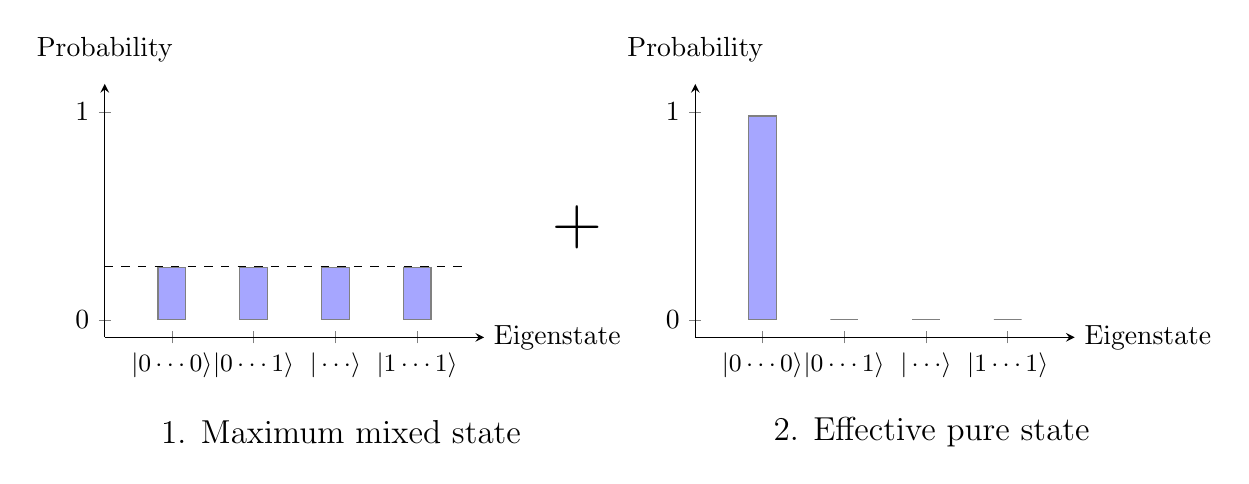
\begin{tikzpicture}

%-----------------------------
% Left plot
%-----------------------------
\begin{axis}[
    at={(0,0)},
    anchor=south west,
    width=6.4cm,
    height=4.8cm,
    axis lines=left,
    ymin=0,ymax=1.05,
    xmin=-0.5,xmax=3.5,
    ytick={0,1},
    xtick={0,1,2,3},
    xticklabels={
        $|0\cdots0\rangle$,
        $|0\cdots1\rangle$,
        $|\cdots\rangle$,
        $|1\cdots1\rangle$
    },
    xticklabel style={font=\small},
    ylabel={Probability},
    xlabel={Eigenstate},
    xlabel style={at={(axis description cs:1,0)},anchor=west},
    y label style={at={(axis description cs:0,1.05)},rotate=-90,anchor=south},
    enlargelimits=0.08,
    clip=false
]

\addplot[
    ybar,
    bar width=10pt,
    draw=black!50,
    fill=blue!35
] coordinates {
    (0,0.25)
    (1,0.25)
    (2,0.25)
    (3,0.25)
};

\end{axis}

\node at (3,-1.2) {\large 1. Maximum mixed state};

%-----------------------------
% Right plot
%-----------------------------
\begin{axis}[
    at={(7.5cm,0)},
    anchor=south west,
    width=6.4cm,
    height=4.8cm,
    axis lines=left,
    ymin=0,ymax=1.05,
    xmin=-0.5,xmax=3.5,
    ytick={0,1},
    xtick={0,1,2,3},
    xticklabels={
        $|0\cdots0\rangle$,
        $|0\cdots1\rangle$,
        $|\cdots\rangle$,
        $|1\cdots1\rangle$
    },
    xticklabel style={font=\small},
    ylabel={Probability},
    xlabel={Eigenstate},
    xlabel style={at={(axis description cs:1,0)},anchor=west},
    ylabel style={at={(axis description cs:0,1.05)},rotate=-90,anchor=south},
    enlargelimits=0.08,
    clip=false
]

\addplot[
    ybar,
    bar width=10pt,
    draw=black!50,
    fill=blue!35
] coordinates {
    (0,0.98)
    (1,0)
    (2,0)
    (3,0)
};

\end{axis}

\draw[dashed] (0,0.9) -- (4.6,0.9);
\node at (10.5,-1.2) {\large 2. Effective pure state};
\node[font=\Huge] at (6.0,1.4) {$+$};

\end{tikzpicture}

\caption{Probability distributions of each component of a pseudo-pure state. The left plot shows the maximum mixed state, in which all states have equal population. The right plot shows the effective pure state, in which only the ground state has population.}
\label{fig:pseudopure}

\end{figure}

This limitation of quantum computing in liquid-state NMR of having to resort to pseudo-pure states is the reason why it is not possible to scale the number of qubits in this platform beyond around ten qubits. The signal intensity decreases exponentially with the number of qubits, making it impossible to measure the result of the computation. The pure fraction of the pseudo-pure state is the state polarization, \(\epsilon\), given by

\begin{equation}
    \epsilon=\frac{2\sinh{(nh\omega/2k_B T)}}{2^n\cosh^n{(h\omega/2k_B T)}}.
    \label{eq:polarization}
\end{equation}

In the high-temperature limit, such as at room temperature, where \(h\omega \ll k_B T\), each additional qubit approximately halves the NMR signal.

\begin{equation}
    \epsilon\approx\frac{nh\omega/2k_B T}{2^n}\approx n 2^{-n}
    \label{eq:polarization_limit}
\end{equation}

As an example, a 100-qubit system at room temperature would produce a signal approximately 28 orders of magnitude below the background noise arising from thermal magnetization, making it impossible to measure. As mentioned previously, cooling the sample to reach a regime in which the signal is not significantly affected, which would be typically around \SI{1}{\kelvin}, depending on the sample, is not feasible, since dipolar couplings re-emerge and spectral lines broaden, among other effects.


\subsection{Preparation methods}
\label{subsec:pseudo_pure_state_preparation}

There are three main methods for preparing a pseudo-pure state. The first, \textbf{Logical labeling with an auxiliary qubit}, makes use of a subset of energy states within the total system whose populations correspond to those required for the pseudo-pure state. In a 3-qubit system, for example, using an auxiliary qubit, the logical states \(\lvert00\rangle\), \(\lvert01\rangle\), \(\lvert10\rangle\), and \(\lvert11\rangle\) of a 2-qubit system are mapped onto four of the eight possible physical states of the 3-qubit system, with these four states sharing the same spin state in the auxiliary qubit, which acts as a label.

The result is a 2-logical-qubit system that exhibits a population distribution corresponding to a pseudo-pure state, to which any logical operations can be applied, provided that the spin of the auxiliary label qubit is not affected. This method is used only in homonuclear systems, since the natural distribution of state populations must follow specific patterns similar to those of a pseudo-pure state in order for them to be labelable.

The second, \textbf{Temporal averaging by permutation}, requires the same algorithm to be run for \(2^n - 1\) initial states, in which the distribution of the excited states is cyclically permuted. The permutation of the excited states is performed by a pulse that repeatedly implements the unitary operation \(P_n\):

\begin{equation}
P_n=\begin{bmatrix}
1 & 0 & 0 & 0 &\cdots & 0 & 0\\
0 & 0 & 0 & 0 &\cdots & 0 & 1\\
0 & 1 & 0 & 0 &\cdots & 0 & 0\\
0 & 0 & 1 & 0 &\cdots & 0 & 0\\
\vdots & \vdots &\vdots & \vdots & \ddots & \vdots & \vdots\\
0 & 0 & 0 & 0 & \cdots & 1 & 0
\end{bmatrix}
\end{equation}

The results are then averaged over the multiple runs. Since the unitary operations that compose the algorithms and the final measurement operations are linear processes, this average is equivalent to the result of the algorithm applied to the average of the initially prepared states.

Finally, the third method, \textbf{Spatial averaging}, is based on adjusting the relative populations of the states by exciting the system, rearranging the populations so that they resemble those of a pseudo-pure state, followed by the use of magnetic field gradients to remove unwanted off-diagonal elements of the density matrix.

The following initialization sequence, adapted from Jones~\cite{Jones2011quantum}, uses a series of rotations to redistribute the state populations, starting from a thermal equilibrium state. This is followed by either a magnetic field gradient that removes the off-diagonal elements of the density matrix, aptly named \emph{crush} gradient, or a period of free evolution under the \(J\)-coupling interaction of duration \(1/(2J)\). The resulting state is a pseudo-pure state.

\begin{equation}
\begin{aligned}
    I_z + S_z &\xrightarrow{60^\circ S_x}I_z + \frac{1}{2}S_z-\frac{\sqrt{3}}{2}S_y \\
    &\xrightarrow{\mathrm{crush}} I_z + \frac{1}{2}S_z\\
    &\xrightarrow{45^\circ I_x} \frac{1}{\sqrt{2}}I_z - \frac{1}{\sqrt{2}}I_y+\frac{1}{2} S_z\\
    &\xrightarrow{\mathrm{J-coupling}} \frac{1}{\sqrt{2}}I_z+\frac{1}{\sqrt{2}}2I_x S_z+\frac{1}{2}S_z\\
    &\xrightarrow{45^\circ I_{-y}} \frac{1}{2}I_z-\frac{1}{2}I_x+\frac{1}{2}2I_x S_z+\frac{1}{2}S_z+\frac{1}{2}2I_z S_z\\
    &\xrightarrow{\mathrm{crush}} \frac{1}{2}I_z+\frac{1}{2}S_z+\frac{1}{2}2I_z S_z\\
\end{aligned}
\label{eq:spatial_averaging}
\end{equation}

Spatial averaging is the most popular method because it does not require additional auxiliary qubits, does not increase the complexity of logical gate design, and is faster than the temporal averaging procedure.

\subsection{Method employed by Gemini}
\label{subsec:gemini_initialization}

The method used for preparing the initial pseudo-pure state in the quantum computer employed in this work is an adaptation of the temporal averaging method. It uses a permutation operation on the excited states followed by a period of longitudinal relaxation of the system, during which the spins are allowed to evolve freely. Repeating this process cyclically causes the populations of the excited states to stabilize at similar values, resulting in a high-fidelity pseudo-pure state.


\begin{figure}[ht]
    \centering
    \begin{tikzpicture}[
    level/.style={line width=1pt},
    pop/.style={circle,fill=gray!70,inner sep=2.6pt},
    permute/.style={
        -{Latex[length=2.5mm]},
        thick,
        black
    },
    relax/.style={
        -{Latex[length=2.5mm]},
        thick,
        blue!70
    }
]

% Legend
\draw[permute] (-1.5,0.4)--(-0.2,0.4);
\node[right] at (-0.1,0.4) {$U_{\mathrm{permute}}$};

\draw[relax] (-1.5,-0.4)--(-0.2,-0.4);
\node[right,align=left] at (-0.1,-0.4)
{Longitudinal\\relaxation};

% LEFT: Thermal equilibrium

\begin{scope}[xshift=4.2cm]

% Energy levels
\draw[level] (0,1.6)--(1.5,1.6);
\draw[level] (-1.5,0.2)--(0,0.2);
\draw[level] (1.5,-0.6)--(3,-0.6);
\draw[level] (0,-2)--(1.5,-2);

% Populations

% |11>
\node[pop] at (0.75,1.85) {};
\node[below] at (0.75,1.55) {$|11\rangle$};

% |10>
\node[pop] at (-0.65,0.45) {};
\node[pop] at (-0.95,0.45) {};
\node[below] at (-0.75,0.15) {$|10\rangle$};

% |01>
\node[pop] at (1.95,-0.35) {};
\node[pop] at (2.25,-0.35) {};
\node[pop] at (2.55,-0.35) {};
\node[below] at (2.25,-0.65) {$|01\rangle$};

% |00>
\node[pop] at (0.35,-1.75) {};
\node[pop] at (0.65,-1.75) {};
\node[pop] at (0.95,-1.75) {};
\node[pop] at (1.25,-1.75) {};
\node[below] at (0.75,-2.05) {$|00\rangle$};

% Curved permutation arrows
% |11> -> |10|  (left side)
\draw[permute]
(-0.15,1.72)
.. controls (-0.85,1.65) and (-0.95,1.10) ..
(-0.75,0.8);

% |10> -> |01|  (bottom)
\draw[permute]
(-0.10,0.10)
.. controls (0.30,-0.60) and (1.10,-0.80) ..
(1.65,-0.68);

% |01> -> |11|  (right side)
\draw[permute]
(2.55,0)
.. controls (3.00,0.30) and (2.90,1.40) ..
(1.45,1.72);

% Relaxation arrows
% |11> -> |10>
\draw[relax]
(0.35,1.40) -- (-0.2,0.30);

% |10> -> |01>
\draw[relax]
(0.1,0.10) -- (1.45,-0.50);

\node at (0.9,-3) {\large Thermal equilibrium state};
\draw[-{Stealth[length=4mm]}, thick](3.8,-3) -- (5.7,-3);

\end{scope}

%Pseudo-pure

\begin{scope}[xshift=11cm]

\draw[level] (0,1.6)--(1.5,1.6);
\draw[level] (-1.5,0.2)--(0,0.2);
\draw[level] (1.5,-0.6)--(3,-0.6);
\draw[level] (0,-2)--(1.5,-2);

\node[pop] at (0.55,1.85) {};
\node[pop] at (0.85,1.85) {};
\node[below] at (0.75,1.55) {$|11\rangle$};

\node[pop] at (-0.65,0.45) {};
\node[pop] at (-0.95,0.45) {};
\node[below] at (-0.75,0.15) {$|10\rangle$};

\node[pop] at (2.05,-0.35) {};
\node[pop] at (2.35,-0.35) {};
\node[below] at (2.25,-0.65) {$|01\rangle$};

\node[pop] at (0.35,-1.75) {};
\node[pop] at (0.65,-1.75) {};
\node[pop] at (0.95,-1.75) {};
\node[pop] at (1.25,-1.75) {};
\node[below] at (0.75,-2.05) {$|00\rangle$};

\node at (0.8,-3) {\large Pseudo pure state};
\end{scope}

\end{tikzpicture}
\label{fig:geminipermutation}
\caption{Initialization process permformed by Gemini to achieve a pseudo-pure state. The populations of the three excited states are cyclically permuted, after which a period of free evolution under solely the \(J\)-coupling interaction is performed. Over time, the populations of the excited states are equalized. Image adapted from SPINQ Gemini Lab manual.}
\end{figure}

\newpage
\section{DiVincenzo 3: Long Decoherence times}
~\label{sec:Divincenzo3}

The main aspect that distinguishes a classical computer from a quantum one is the ability of qubits to exist in a state of superposition, enabling the processing of more information more rapidly and being essential for more complex algorithms. However, superposition cannot be maintained indefinitely. Both experimental measurements and interactions with the external environment cause a quantum state to lose coherence over time.

The coherence time of a state depends on the architecture used for the quantum computer and corresponds to the maximum time allowed for the implementation of algorithms. Naturally, quantum logic gates must have durations limited by these values so that they can act before the onset of decoherence.

\subsection{Longitudinal Relaxation}
\label{subsec:longitudinal_relaxation}

Through spin-lattice relaxation, the longitudinal component of the nuclear spin, parallel to the direction of the magnetic field, relaxes from a higher-energy state toward the thermodynamic equilibrium state via interaction with the environment. The expected value of \(\langle S_z\rangle\) evolves according to the exponential law

\begin{equation}
    \langle S_z\rangle(t)=\langle S_z\rangle_0+(\langle S_z\rangle_{eq}-\langle S_z\rangle_0)(1-e^{-\frac{t}{T_1}}).
    \label{eq:T1_relaxation}
\end{equation}

\begin{figure}[htb]
\centering
\begin{tikzpicture}
    \begin{axis}[
    width=9cm,
    height=6cm,
    xmin=0, xmax=5,
    ymin=0, ymax=1,
    xlabel={$t/T_1$},
    ylabel={$\langle S_z\rangle(t)$},
    axis lines=left,
    xtick={0,1,2,3,4},
    ytick={0,0.8},
    yticklabels={
        $\langle S_z\rangle_0$,
        $\langle S_z\rangle_{eq}$
    },
    samples=200,
    domain=0:5,
    clip=false
]

% Parameters:
% <Sz>_0 = 0
% <Sz>_eq = 0.8
\addplot[
    thick,
    blue
]
{0 + (0.8)*(1-exp(-x))};

% Initial point
\addplot[only marks,mark=*,blue]
coordinates {(0,0)};

% Equilibrium line
\addplot[
    dashed,
    gray
]
coordinates {(0,0.8) (5,0.8)};
\end{axis}

\end{tikzpicture}
\caption{Evolution of $\langle S_z\rangle(t)$. The longitudinal component of the nuclear spin behaves as a magnetic dipole that relaxes toward an equilibrium state, which in this case is the alignment with the external magnetic field.}
\label{fig:longitudinalrelaxation}
\end{figure}

\begin{figure}[htb]
\centering
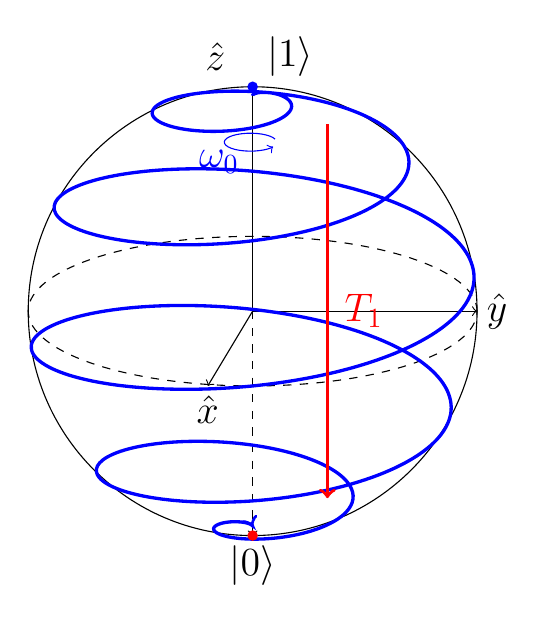
\begin{tikzpicture}[scale=0.95,font=\Large]

\def\r{3}
\def\a{0.85}

% Sphere
\draw (0,0) circle(\r);
\draw[dashed] (0,0) ellipse({\r} and {\r/3});

% Axes
\draw[->] (0,0)--(\r,0) node[right]{$\hat y$};
\draw[->] (0,0)--(0,\r) node at (-0.5,\r+0.4){$\hat z$};
\draw[->] (0,0)--(-0.6,-1) node[below]{$\hat x$};
\draw[dashed,->] (0,0) -- ++(0,-\r) node[below] {$|0\rangle$};

% Basis states
\node at (0.5,\r+0.4){$|1\rangle$};

% Number of revolutions
\def\nturns{5}

% Spiral on the surface
\def\eps{0.96}
\def\delta{0.04}

\draw[
    very thick,
    blue,
    samples=400,
    smooth,
    domain=0:1,
    variable=\u,
    ->]
plot
(
{
\r*(\eps+\delta*sin(180*\u)^2)
*sin(180*\u)
*sin(360*\nturns*\u)
},
{
\r*(\eps+\delta*sin(180*\u)^2)
*cos(180*\u)
+
(\r/3)*(\eps+\delta*sin(180*\u)^2)
*sin(180*\u)
*cos(360*\nturns*\u)
}
);

% Initial point
\fill[blue] (0,\r) circle(2pt);

% Final point
\fill[red] (0,-\r) circle(2pt);

% T1 arrow
\draw[red,very thick,->]
(1.0,2.5)--(1.0,-2.5);

\node[red,right] at (1.1,0){$T_1$};

%Precession
\draw[blue,->]
(0.30,\r-0.7)
arc[start angle=20,end angle=330,x radius=.35,y radius=.12];

\node[blue] at (-.45,\r-1.0){$\omega_0$};

\end{tikzpicture}
\label{fig:bloch_longitudinal}
\caption{Bloch sphere representation of Longitudinal relaxation. While the longitudinal component of the nuclear spin relaxes from the excited state $|1\rangle$ toward the equilibrium state $|0\rangle$, the transverse component precesses around the external magnetic field at the Larmor frequency.}
\end{figure}

In this expression, \(\langle S_z\rangle_0\) is the initial state of the longitudinal spin component before relaxation, and \(\langle S_z\rangle_{eq}\) is the component corresponding to maximum decoherence, i.e., the equilibrium state. The characteristic constant \(T_1\) determines the rate of the relaxation process, with larger values of \(T_1\) corresponding to slower relaxation and therefore more time available to implement the desired algorithms.

Its measurement can be easily performed by repeatedly exciting each qubit from the \(\lvert 0 \rangle\) state to the \(\lvert 1 \rangle\) state, allowing it to evolve freely, and measuring the \(\langle S_z \rangle\) component of the state at different time intervals. The curve~\ref{eq:T1_relaxation} is then fitted to the set of results, yielding a value for \(T_1\).

\subsection{Transverse Relaxation}
\label{subsec:transverse_relaxation}

Through spin–spin relaxation, the transverse component of the nuclear spin relaxes toward the equilibrium state, leading to the loss of phase information and of the state’s superposition. This component, \(\langle S_{xy}\rangle\), similarly evolves according to the exponential law

\begin{equation}
    \langle S_{xy}\rangle(t)=\langle S_{xy}\rangle_0e^{-\frac{t}{T_2}}.
    \label{eq:T2_relaxation}
\end{equation}


\begin{figure}[ht]
\centering
\begin{tikzpicture}
\begin{axis}[
    width=10cm,
    height=6cm,
    xmin=0, xmax=5,
    ymin=0, ymax=1.1,
    axis lines=left,
    xlabel={$t$},
    ylabel={$\langle S_{xy}\rangle(t)$},
    xtick={0},
    xticklabels={$0$},
    ytick={0,0.368,1},
    yticklabels={$0$,$e^{-1}\langle S_{xy}\rangle_0$,$\langle S_{xy}\rangle_0$},
    domain=0:5,
    samples=200,
    clip=false
]

% Exponential decay
\addplot[blue,very thick] {exp(-x/2)};

% Dashed guides at T2
\addplot[dashed] coordinates {(2,0) (2,{exp(-1)})};
\addplot[dashed] coordinates {(0,{exp(-1)}) (2,{exp(-1)})};

% Initial point
\addplot[only marks,mark=*,blue] coordinates {(0,1)};

% T2 annotation
\node[below] at (axis cs:2,0) {$T_2$};

\end{axis}
\end{tikzpicture}

\caption{Evolution of $\langle S_{xy}\rangle(t)$. The transverse component of the nuclear spin relaxes toward the equilibrium state, leading to the loss of information. The relaxation rate is characterized by a time constant: \(T_2\).}
\label{fig:transverserelaxation}
\end{figure}

\begin{figure}[ht]
\centering
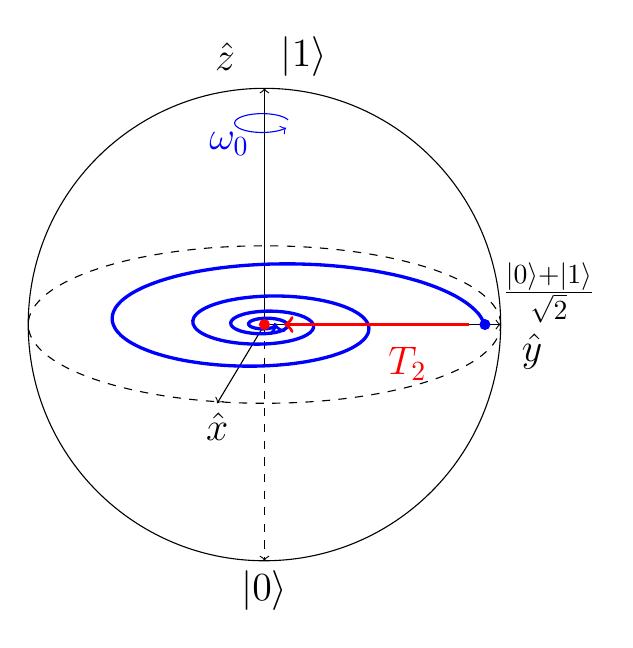
\begin{tikzpicture}[scale=1,font=\Large]

\def\r{3}
\def\a{2.8}
\def\k{0.08}

% Sphere
\draw (0,0) circle(\r);
\draw[dashed] (0,0) ellipse({\r} and {\r/3});

% Axes
\draw[->] (0,0)--(\r,0) node[below] at (3.4,0){$\hat y$};
\draw[->] (0,0)--(0,\r) node at (-0.5,\r+0.4){$\hat z$};
\draw[->] (0,0)--(-0.6,-1) node[below]{$\hat x$};
\draw[dashed,->] (0,0) -- ++(0,-\r) node[below] {$|0\rangle$};

% Basis states
\node at (0.5,\r+0.4){$|1\rangle$};

% Initial state label
\node[right] at (2.9,.4)
{$\frac{|0\rangle+|1\rangle}{\sqrt2}$};

% Inward spiral
\draw[very thick,blue,samples=180,smooth,domain=0:8*pi,variable=\t,->]
plot
(
{\a*exp(-0.12*\t)*cos(\t r)},
{0.33*\a*exp(-0.12*\t)*sin(\t r)}
);

% Initial point
\fill[blue] (\a,0) circle(2pt);

% Origin
\fill[red] (0,0) circle(2pt);

% T2 label
\draw[red,very thick,->]
(2.6,0)--(.25,0);

\node[red,right] at (1.45,-0.5){$T_2$};

%Precession
\draw[blue,->]
(0.30,\r-0.4)
arc[start angle=20,end angle=330,x radius=.35,y radius=.12];

\node[blue] at (-.45,\r-0.7){$\omega_0$};

\end{tikzpicture}
\label{fig:bloch_transverse}
\caption{Bloch sphere representation of Transverse relaxation. The transverse component of the nuclear spin relaxes from an example superposition state \(\frac{1}{\sqrt{2}}(|0\rangle + |1\rangle)\), toward the equilibrium maximum mixed state, losing phase information and coherence. The precession around the external magnetic field continues at the Larmor frequency.}
\end{figure}

The relaxation rate is, similarly to longitudinal relaxation, characterized by a time constant \(T_2\). \(T_2\) relaxation is generally faster than \(T_1\) relaxation, and is therefore the limiting factor.

As with \(T_1\), the characteristic constant \(T_2\) is measured by fitting the curve~\ref{eq:T2_relaxation} to a set of data points obtained by initializing the system in the state \(\frac{1}{\sqrt{2}}(\lvert0\rangle+\lvert1\rangle)\). During free evolution, \(R_x(\pi)\) pulses are applied at \(t/2\) and \(t\), implementing the spin echo technique to reduce additional external effects on the qubit, such as coupling, magnetic field inhomogeneity, and noise. Due to the spatial distribution of molecules in the sample within the magnetic field, any inhomogeneity in the field causes a difference in the precession frequency around the field axis. These differences accumulate phase variations that reduce the coherence of the state.

The effect of the \(R_x(\pi)\) pulses is, in approximation, to cancel the errors introduced by these factors on average, by flipping the direction of the longitudinal evolution.

The Rabi relaxation time, \(T_2^*\), is further defined, corresponding to the same type of transverse relaxation as \(T_2\), but in the absence of spin echo pulses. It represents the relaxation of the \(\langle S_{xy}\rangle\) component when it is also affected by factors such as those mentioned previously, and can be considered the limit of system coherence in the worst-case scenario.

\subsection{Time requirements}
\label{subsec:time_requirements}

According to DiVincenzo, relaxation times should be \(10^4\) to \(10^5\) times longer than quantum gate operation times. In the two-qubit sample system used in the Gemini Lab quantum computer, we measure \(T_1 \approx 11\,\text{s}\) and \(T_2 \approx 4\,\text{s}\). The \(J\)-coupling interaction used to implement two-qubit gates imposes minimum gate durations on the order of milliseconds. This requirement is therefore satisfied.

However, reducing the duration of the designed quantum gates remains an important objective in pulse sequence optimization.


\section{DiVincenzo 4: Universal set of Quantum Gates}
~\label{sec:Divincenzo4}

To use the two-level system that defines each qubit, it is necessary to be able to transform the system from any initial state \(\psi_0\) to any target state \(\psi_1\). Formally, quantum gate universality is the ability to achieve any desired evolution using a finite set of quantum gates.

There are several possible universal sets of quantum gates. The most common choice consists of single-qubit rotations, together with any non-trivial two-qubit gate, i.e., a gate that cannot be decomposed into independent single-qubit rotations. Such gates typically rely on an intrinsic coupling interaction between two qubits in the system.

In NMR, as a consequence of the system model given by Eq.~\ref{eq:full_Hamiltonian} and described in Section~\ref{sec:Divincenzo1}, any single-qubit rotation can be implemented through the control Hamiltonian term, since it has components along \(I_x\) and \(I_y\). Rotations about the \(\hat{x}\) and \(\hat{y}\) axes are achieved using pulses that differ only in phase, while rotations about the \(\hat{z}\) axis can be implemented either through free precession around the constant field direction \(\vec{B_0}\), or, equivalently, by decomposing them into rotations about transverse axes.

Using Euler angle decomposition, an arbitrary single-qubit rotation can be expressed as a sequence of rotations about two orthogonal axes in the transverse plane (e.g., \(\hat{x}\) and \(\hat{y}\)), such as \(R_x(\alpha)R_y(\beta)R_x(\gamma)\), which reproduces any effective rotation including those about \(\hat{z}\). The \(J\)-coupling term is used for the implementation of multi-qubit gates.

\begin{figure}[ht]
\centering
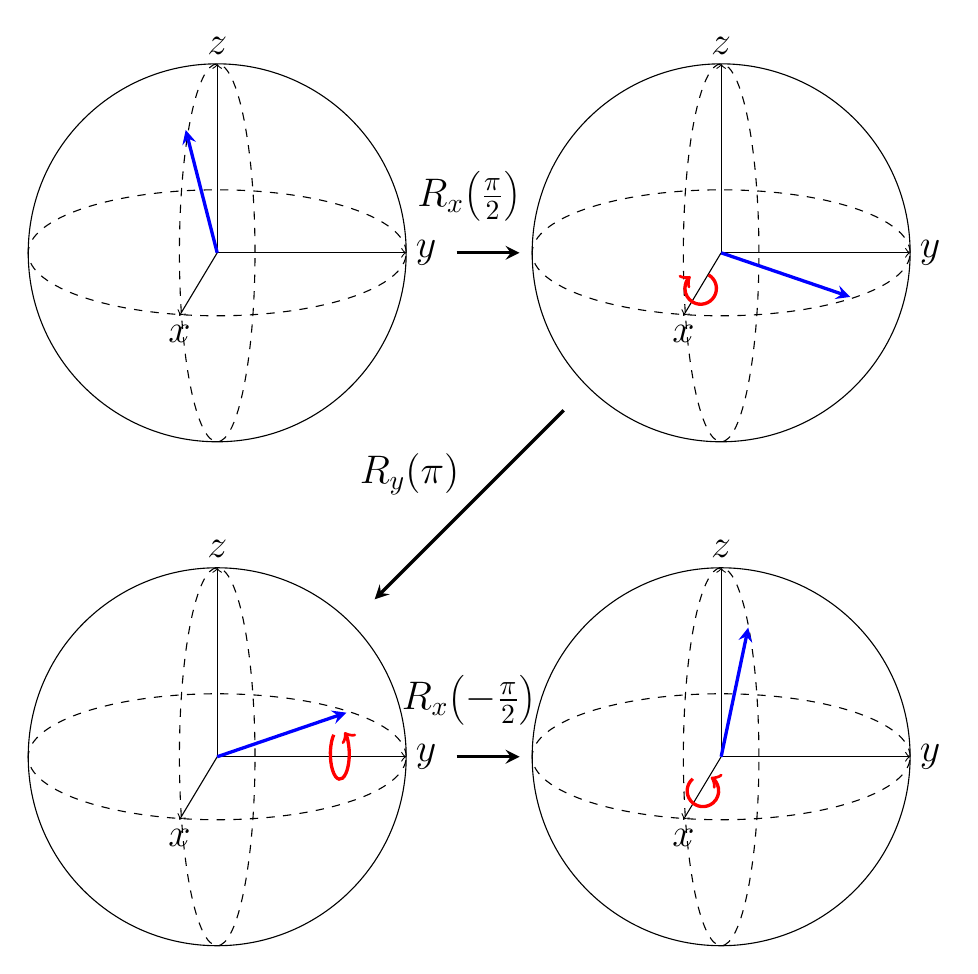
\begin{tikzpicture}[scale=0.8,font=\Large]

\def\r{3}

%====================================================
% Sphere 0 : Initial state
%====================================================
\begin{scope}[shift={(0,0)}]

% Sphere
\draw (0,0) circle(\r);
\draw[dashed] (0,0) ellipse ({\r} and {\r/3});
\draw[dashed] (0,0) ellipse ({\r/5} and {\r});

% Axes
\draw[->] (0,0)--(0,\r) node[above]{$z$};
\draw[->] (0,0)--(\r,0) node[right]{$y$};
\draw[->] (0,0)--(-\r/5,-\r/3) node[below]{$x$};

% State vector
\draw[very thick,blue,-stealth] (0,0)--(-0.5,1.95);

\end{scope}
%====================================================
% Sphere 1 : Rx(alpha)
%====================================================
\begin{scope}[shift={(8,0)}]

% Sphere
\draw (0,0) circle(\r);
\draw[dashed] (0,0) ellipse ({\r} and {\r/3});
\draw[dashed] (0,0) ellipse ({\r/5} and {\r});

% Axes
\draw[->] (0,0)--(0,\r) node[above]{$z$};
\draw[->] (0,0)--(\r,0) node[right]{$y$};
\draw[->] (0,0)--(-\r/5,-\r/3) node[below]{$x$};

% State vector
\draw[very thick,blue,-stealth] (0,0)--(2.05,-0.7);

% Rotation arrow about x
\draw[red,very thick,->]
(-0.2,-0.35)
arc[start angle=420,end angle=130,
x radius=.25,
y radius=.25];

\end{scope}

%====================================================
% Sphere 2 : Ry(beta)
%====================================================
\begin{scope}[shift={(0,-8)}]

\draw (0,0) circle(\r);
\draw[dashed] (0,0) ellipse ({\r} and {\r/3});
\draw[dashed] (0,0) ellipse ({\r/5} and {\r});

\draw[->] (0,0)--(0,\r) node[above]{$z$};
\draw[->] (0,0)--(\r,0) node[right]{$y$};
\draw[->] (0,0)--(-\r/5,-\r/3) node[below]{$x$};

% Rotated state
\draw[very thick,blue,-stealth] (0,0)--(2.05,0.7);

% Rotation arrow about y

\draw[red,very thick,->]
(1.85,0.35)
arc[start angle=130,end angle=420,
x radius=.15,
y radius=.4];

\end{scope}

%====================================================
% Sphere 3 : Rx(gamma)
%====================================================
\begin{scope}[shift={(8,-8)}]

\draw (0,0) circle(\r);
\draw[dashed] (0,0) ellipse ({\r} and {\r/3});
\draw[dashed] (0,0) ellipse ({\r/5} and {\r});

\draw[->] (0,0)--(0,\r) node[above]{$z$};
\draw[->] (0,0)--(\r,0) node[right]{$y$};
\draw[->] (0,0)--(-\r/5,-\r/3) node[below]{$x$};

% Final state
\draw[very thick,blue,-stealth] (0,0)--(0.43,2.05);

% Rotation arrow about x
\draw[red,very thick,->]
(-0.45,-0.35)
arc[start angle=130,end angle=420,
x radius=.25,
y radius=.25];

\end{scope}

%Arrows
% Sphere 0 -> Sphere 1
\draw[very thick,-stealth] (3.8,0)--(4.8,0);
\node[above] at (4,0.35)
{$R_x\!\left(\frac{\pi}{2}\right)$};

% Sphere 1 -> Sphere 2
\draw[very thick,-stealth] (5.5,-2.5)--(2.5,-5.5);
\node[above left] at (4,-4)
{$R_y(\pi)$};

% Sphere 2 -> Sphere 3
\draw[very thick,-stealth] (3.8,-8)--(4.8,-8);
\node[above] at (4,-7.65)
{$R_x\!\left(-\frac{\pi}{2}\right)$};


\end{tikzpicture}
\caption{An arbitrary single-qubit rotation can be decomposed into three successive rotations about the $x$ and $y$ axes. Here, the rotation $R_z(\pi)$ is implemented using the Euler decomposition $R_z(\pi)=R_x\!\left(\frac{\pi}{2}\right)R_y(\pi)R_x\!\left(-\frac{\pi}{2}\right)$, illustrating the evolution of the Bloch vector after each elementary rotation.}
\label{fig:RxRyRx}
\end{figure}

An important point to consider is that the implementation of some of these gates requires spin-selective excitation. As mentioned previously, in heteronuclear systems the different nuclei have significantly distinct Larmor precession frequencies. This makes each qubit easily identifiable and individually addressable in the frequency domain.

In homonuclear systems, the Larmor frequencies of different qubits are very close to each other, making them difficult to distinguish in the frequency domain. Nevertheless, small variations in these frequencies arise due to the electronic environment and the molecular geometry, known as chemical shifts. When these differences are sufficiently large, they can be exploited to design selective pulses capable of acting on specific qubits.

When a clear separation cannot be achieved through chemical shifts, the multi-qubit system must be manipulated collectively, taking into account the joint behavior of the entire system.

\begin{figure}[ht]
\centering
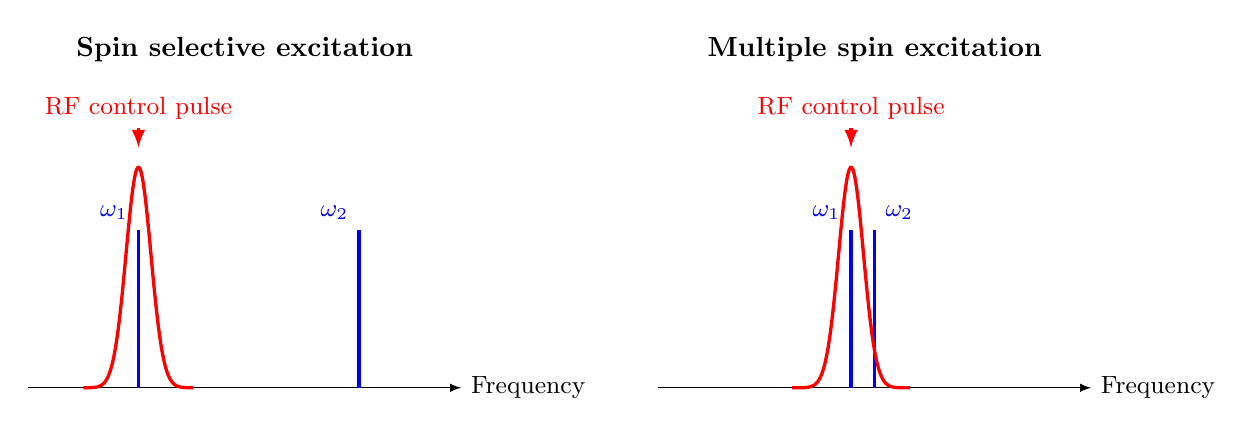
\begin{tikzpicture}[>=latex,font=\small]

%------------------------------------------------
% LEFT: Selective spin
%------------------------------------------------
\begin{scope}

\node[font=\bfseries] at (2.75,4.3) {Spin selective excitation};

% Frequency axis
\draw[->] (0,0)--(5.5,0) node[right]{Frequency};

% Resonances
\draw[very thick,blue] (1.4,0)--(1.4,2) node[above left]{$\omega_1$};
\draw[very thick,blue] (4.2,0)--(4.2,2) node[above left]{$\omega_2$};

%RF pulse
\draw[red,very thick,samples=100,smooth,domain=0.7:2.1]
plot(\x,{2.8*exp(-20*(\x-1.4)^2)});

\draw[red,very thick,->] (1.4,3.3)--(1.4,3.05);

\node[red] at (1.4,3.55){RF control pulse};

\end{scope}

%------------------------------------------------
% RIGHT: Multiple spins
%------------------------------------------------
\begin{scope}[xshift=8cm]

\node[font=\bfseries] at (2.75,4.3) {Multiple spin excitation};

% Frequency axis
\draw[->] (0,0)--(5.5,0) node[right]{Frequency};

% Nearly overlapping resonances
\draw[very thick,blue] (2.45,0)--(2.45,2) node[above left]{$\omega_1$};
\draw[very thick,blue] (2.75,0)--(2.75,2) node[above right]{$\omega_2$};

%RF pulse
\draw[red,very thick,samples=100,smooth,domain=1.7:3.2]
plot(\x,{2.8*exp(-20*(\x-2.45)^2)});

\draw[red,very thick,->] (2.45,3.3)--(2.45,3.05);

\node[red] at (2.45,3.55){RF control pulse};

\end{scope}

\end{tikzpicture}
\caption{Selective and collective excitation in NMR systems. A radio frequency control pulse excites only the resonant nuclei when the Larmor frequencies are separated by a sufficiently large margin (left). When the frequencies are close to each other, the pulse overlaps nearby resonances causing partial excitation. This effect occurs in homonuclear systems when the chemical shift is too small (right).}
\label{fig:chemical_shift_gaussian}
\end{figure}


\section{DiVincenzo 5: Individual measurement} 
~\label{sec:Divincenzo5}

\subsection{Free Induction Decay}
\label{subsec:FID}

The measurement of each qubit state is not performed by directly measuring individual nuclear spins. The quantum system is an ensemble of approximately \(10^{23}\) molecules, each containing as many relevant nuclear spins as there are nuclei used as qubits. The measured quantity is, instead, the macroscopic magnetic moment of the system, \(\hat{M}=(M_x,M_y,M_z)\), whose components are proportional to the statistical average of the corresponding spin components \(\langle S_x\rangle,\langle S_y\rangle,\langle S_z\rangle\), i.e., the nuclear spin angular momentum.

Thus, when referring to the state of a qubit, one is not describing the spin state of a single molecule, but rather the ensemble average \(\hat{M}\).

When an RF field is applied at the same frequency as the intrinsic precession frequency of the qubit spin, \(\omega_0\), i.e., its Larmor frequency, the energy of the field matches the energy difference between the qubit levels. During this resonance between the field and the qubit, the latter can absorb energy and transition from the lower-energy state to the excited state, resulting in a rotation of the \(M_z\) component toward the negative direction of the \(\hat{z}\) axis, or, via stimulated emission, undergo the reverse process.

Simultaneously, the transverse component of the net magnetic moment precesses around the axis of the static magnetic field \(\vec{B_0}\) at frequency \(\omega_0\), as it reflects the ensemble average behavior of each nuclear spin as described in Section~\ref{sec:Divincenzo1}. The time evolution of the \(M_x\) and \(M_y\) components, also including decoherence effects, can be expressed as

\begin{equation}
\begin{aligned}
M_x(t) &= \lvert M_{xy}(t_0)\rvert \cos\! \bigl(2\pi\omega_0 t+\phi\bigr)e^{-t/T_2}, \\
M_y(t) &= \lvert M_{xy}(t_0)\rvert \sin\!\bigl(2\pi\omega_0 t+\phi\bigr)e^{-t/T_2}.
\label{eq:net_magnetic_moment}
\end{aligned}
\end{equation}

\begin{figure}[ht]
    \centering
    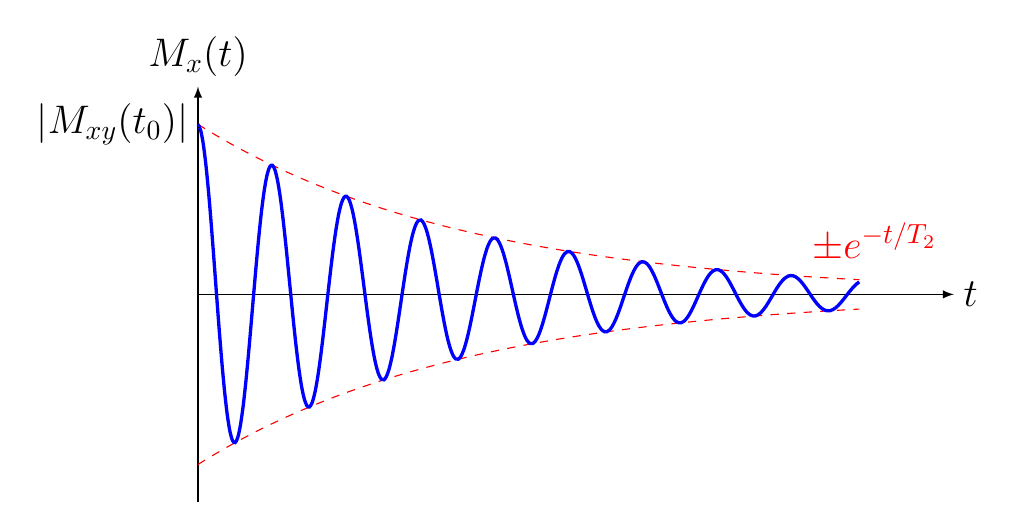
\begin{tikzpicture}[scale=1.2,>=latex,font=\Large]

% Axes
\draw[->] (0,0) -- (8,0) node[right] {$t$};
\draw[->] (0,-2.2) -- (0,2.2) node[above] {$M_x(t)$};

% Exponential envelopes
\draw[dashed,red,domain=0:7,samples=100,smooth]
plot (\x,{1.8*exp(-0.35*\x)});

\draw[dashed,red,domain=0:7,samples=100,smooth]
plot (\x,{-1.8*exp(-0.35*\x)});

\node[red,right] at (6.4,0.55) {$\pm e^{-t/T_2}$};

% FID signal
\draw[very thick,blue,domain=0:7,samples=250,smooth]
plot (\x,{1.8*exp(-0.35*\x)*cos(deg(8*\x))});

% Initial amplitude
\draw[dotted] (0,0)--(0,1.8);
\node[left] at (0,1.8) {$|M_{xy}(t_0)|$};

\end{tikzpicture}
\caption{Free induction decay (FID) generated by the transverse magnetization after RF excitation. The detected signal oscillates at the Larmor frequency $\omega_0$ while its amplitude decays exponentially with the transverse relaxation time $T_2$, as described by the exponentially damped transverse magnetization.}
\label{fig:FID}
\end{figure}

The evolution of the transverse component of the magnetic moment generates an electromagnetic field that is detected by the system’s coils, known as the Free Induction Decay (FID), which contains the information required to reconstruct the initial quantum state.

The frequency-domain counterpart of the FID signal, obtained via a Fourier transform, is referred to as a Complex Lorentzian. The magnitudes of these frequency-domain signals are proportional to the values of the \(M_x\) and \(M_y\) components prior to the onset of relaxation. To measure \(M_z\), the quantum state is rotated so that it is mapped onto the \(M_x\) axis, after which it is measured in the same manner.

\subsection{Quantum state tomography}
\label{subsec:quantum_state_tomography}

Quantum state tomography is the process of reconstructing a quantum state utilizing information from multiple diferent measurements of identical states. These measurements must use operators that form a complete basis on the Hilbert space of the system, so that the full density matrix can be reconstructed. 

Realizing quantum tomography on the state of a single qubit is simple. The density matrix can be fully reconstructed using the Pauli operators, which translate to measuring the Bloch vector, \(\vec{r}\), in the directions \(\hat{x},\hat{y},\hat{z}\). The process of measurement causes the collapse of the quantum state onto one of the possible eigenstates. This is a probabilistic outcome, so multiple measurements of the same observable can be conducted to recover the initial component of the Bloch vector in its direction. 

\begin{equation}
\rho = \frac{1}{2}\left(I + \vec{r}\cdot\vec{\sigma}\right)
= \frac{1}{2}
\begin{bmatrix}
1 + r_z & r_x - i r_y \\
r_x + i r_y & 1 - r_z
\end{bmatrix}
\end{equation}

However, quantum tomography of multi-qubit systems isn't that simple. As the number of qubits increases, the number of observables required to reconstruct the density matrix also increases, and finding measurement basis that provide information efficiently can be challenging. In addition, the possibility of quantum entanglement existing between two qubits prevents the reconstruction of the complete quantum state of a composite system from separate qubit measurements.

In that case, the Complex Lorentzian resulting from the Fourier transform of the Free Induction Decay signal previously mentioned must be studied.

\begin{equation}
\begin{aligned}
L_{M_x} &= \frac{\lvert a_l \rvert[\cos{(\phi)}\lambda+\sin{(\phi)}(\omega-\omega_0)]}{\lambda^2+{(\omega-\omega_0)}^2}\\
L_{M_y} &= \frac{\lvert a_l \rvert[\sin{(\phi)}\lambda+\cos{(\phi)}(\omega-\omega_0)]}{\lambda^2+{(\omega-\omega_0)}^2}
\end{aligned}
\label{eq:complex_lorentzian}
\end{equation}


% Elaborate on complex lorentzian